\documentclass[openany]{book}
\usepackage{lmodern}
\usepackage{amssymb,amsmath}
\usepackage{ifxetex,ifluatex}
\usepackage{fixltx2e} % provides \textsubscript
\ifnum 0\ifxetex 1\fi\ifluatex 1\fi=0 % if pdftex
  \usepackage[T1]{fontenc}
  \usepackage[utf8]{inputenc}
\else % if luatex or xelatex
  \ifxetex
    \usepackage{mathspec}
  \else
    \usepackage{fontspec}
  \fi
  \defaultfontfeatures{Ligatures=TeX,Scale=MatchLowercase}
\fi
% use upquote if available, for straight quotes in verbatim environments
\IfFileExists{upquote.sty}{\usepackage{upquote}}{}
% use microtype if available
\IfFileExists{microtype.sty}{%
\usepackage{microtype}
\UseMicrotypeSet[protrusion]{basicmath} % disable protrusion for tt fonts
}{}
\usepackage[margin=1in]{geometry}
\usepackage{hyperref}
\hypersetup{unicode=true,
            pdftitle={Singapore Society in Numbers},
            pdfauthor={Edited by Shannon Ang},
            pdfborder={0 0 0},
            breaklinks=true}
\urlstyle{same}  % don't use monospace font for urls
\usepackage{natbib}
\bibliographystyle{apalike}
\usepackage{color}
\usepackage{fancyvrb}
\newcommand{\VerbBar}{|}
\newcommand{\VERB}{\Verb[commandchars=\\\{\}]}
\DefineVerbatimEnvironment{Highlighting}{Verbatim}{commandchars=\\\{\}}
% Add ',fontsize=\small' for more characters per line
\usepackage{framed}
\definecolor{shadecolor}{RGB}{248,248,248}
\newenvironment{Shaded}{\begin{snugshade}}{\end{snugshade}}
\newcommand{\KeywordTok}[1]{\textcolor[rgb]{0.13,0.29,0.53}{\textbf{#1}}}
\newcommand{\DataTypeTok}[1]{\textcolor[rgb]{0.13,0.29,0.53}{#1}}
\newcommand{\DecValTok}[1]{\textcolor[rgb]{0.00,0.00,0.81}{#1}}
\newcommand{\BaseNTok}[1]{\textcolor[rgb]{0.00,0.00,0.81}{#1}}
\newcommand{\FloatTok}[1]{\textcolor[rgb]{0.00,0.00,0.81}{#1}}
\newcommand{\ConstantTok}[1]{\textcolor[rgb]{0.00,0.00,0.00}{#1}}
\newcommand{\CharTok}[1]{\textcolor[rgb]{0.31,0.60,0.02}{#1}}
\newcommand{\SpecialCharTok}[1]{\textcolor[rgb]{0.00,0.00,0.00}{#1}}
\newcommand{\StringTok}[1]{\textcolor[rgb]{0.31,0.60,0.02}{#1}}
\newcommand{\VerbatimStringTok}[1]{\textcolor[rgb]{0.31,0.60,0.02}{#1}}
\newcommand{\SpecialStringTok}[1]{\textcolor[rgb]{0.31,0.60,0.02}{#1}}
\newcommand{\ImportTok}[1]{#1}
\newcommand{\CommentTok}[1]{\textcolor[rgb]{0.56,0.35,0.01}{\textit{#1}}}
\newcommand{\DocumentationTok}[1]{\textcolor[rgb]{0.56,0.35,0.01}{\textbf{\textit{#1}}}}
\newcommand{\AnnotationTok}[1]{\textcolor[rgb]{0.56,0.35,0.01}{\textbf{\textit{#1}}}}
\newcommand{\CommentVarTok}[1]{\textcolor[rgb]{0.56,0.35,0.01}{\textbf{\textit{#1}}}}
\newcommand{\OtherTok}[1]{\textcolor[rgb]{0.56,0.35,0.01}{#1}}
\newcommand{\FunctionTok}[1]{\textcolor[rgb]{0.00,0.00,0.00}{#1}}
\newcommand{\VariableTok}[1]{\textcolor[rgb]{0.00,0.00,0.00}{#1}}
\newcommand{\ControlFlowTok}[1]{\textcolor[rgb]{0.13,0.29,0.53}{\textbf{#1}}}
\newcommand{\OperatorTok}[1]{\textcolor[rgb]{0.81,0.36,0.00}{\textbf{#1}}}
\newcommand{\BuiltInTok}[1]{#1}
\newcommand{\ExtensionTok}[1]{#1}
\newcommand{\PreprocessorTok}[1]{\textcolor[rgb]{0.56,0.35,0.01}{\textit{#1}}}
\newcommand{\AttributeTok}[1]{\textcolor[rgb]{0.77,0.63,0.00}{#1}}
\newcommand{\RegionMarkerTok}[1]{#1}
\newcommand{\InformationTok}[1]{\textcolor[rgb]{0.56,0.35,0.01}{\textbf{\textit{#1}}}}
\newcommand{\WarningTok}[1]{\textcolor[rgb]{0.56,0.35,0.01}{\textbf{\textit{#1}}}}
\newcommand{\AlertTok}[1]{\textcolor[rgb]{0.94,0.16,0.16}{#1}}
\newcommand{\ErrorTok}[1]{\textcolor[rgb]{0.64,0.00,0.00}{\textbf{#1}}}
\newcommand{\NormalTok}[1]{#1}
\usepackage{longtable,booktabs}
\usepackage{graphicx,grffile}
\makeatletter
\def\maxwidth{\ifdim\Gin@nat@width>\linewidth\linewidth\else\Gin@nat@width\fi}
\def\maxheight{\ifdim\Gin@nat@height>\textheight\textheight\else\Gin@nat@height\fi}
\makeatother
% Scale images if necessary, so that they will not overflow the page
% margins by default, and it is still possible to overwrite the defaults
% using explicit options in \includegraphics[width, height, ...]{}
\setkeys{Gin}{width=\maxwidth,height=\maxheight,keepaspectratio}
\IfFileExists{parskip.sty}{%
\usepackage{parskip}
}{% else
\setlength{\parindent}{0pt}
\setlength{\parskip}{6pt plus 2pt minus 1pt}
}
\setlength{\emergencystretch}{3em}  % prevent overfull lines
\providecommand{\tightlist}{%
  \setlength{\itemsep}{0pt}\setlength{\parskip}{0pt}}
\setcounter{secnumdepth}{5}
% Redefines (sub)paragraphs to behave more like sections
\ifx\paragraph\undefined\else
\let\oldparagraph\paragraph
\renewcommand{\paragraph}[1]{\oldparagraph{#1}\mbox{}}
\fi
\ifx\subparagraph\undefined\else
\let\oldsubparagraph\subparagraph
\renewcommand{\subparagraph}[1]{\oldsubparagraph{#1}\mbox{}}
\fi

%%% Use protect on footnotes to avoid problems with footnotes in titles
\let\rmarkdownfootnote\footnote%
\def\footnote{\protect\rmarkdownfootnote}

%%% Change title format to be more compact
\usepackage{titling}

% Create subtitle command for use in maketitle
\providecommand{\subtitle}[1]{
  \posttitle{
    \begin{center}\large#1\end{center}
    }
}

\setlength{\droptitle}{-2em}

  \title{Singapore Society in Numbers}
    \pretitle{\vspace{\droptitle}\centering\huge}
  \posttitle{\par}
    \author{Edited by Shannon Ang}
    \preauthor{\centering\large\emph}
  \postauthor{\par}
      \predate{\centering\large\emph}
  \postdate{\par}
    \date{Last updated 22 May 2019}

\usepackage{booktabs}
\usepackage{amsthm}
\makeatletter
\def\thm@space@setup{%
  \thm@preskip=8pt plus 2pt minus 4pt
  \thm@postskip=\thm@preskip
}
\makeatother

\begin{document}
\maketitle

{
\setcounter{tocdepth}{1}
\tableofcontents
}
\chapter*{Preface}\label{preface}
\addcontentsline{toc}{chapter}{Preface}

This online book is a compilation of resources aimed at advancing
quantitative social science in Singapore. It is meant to be a `living
document', so it will be updated as frequently as possible. The main
goal is to promote interest, rigour, and transparency in trying to
understand Singapore society quantitatively. It does so by:

\begin{enumerate}
\def\labelenumi{\arabic{enumi}.}
\tightlist
\item
  \textbf{Providing information on Singapore-relevant datasets} that are
  currently used to answer research and policy questions (Chapter
  \ref{publicdata} and Chapter \ref{restricteddata}). This includes:

  \begin{itemize}
  \tightlist
  \item
    Descriptions of \emph{publicly available} datasets and how to access
    them. This overview of the `data landscape' will be helpful for
    social scientists to get started with research on Singapore, and
    prevent wasteful overlap in primary data collection across
    institutions.
  \item
    A list of \emph{restricted} or \emph{non-publicly available}
    datasets that could be used to answer important research or policy
    questions if access was granted. If available, details on the
    dataset and reasons for data restriction will also be listed. It is
    hoped that this list will promote greater transparency in data
    sharing across research teams.
  \end{itemize}
\item
  \textbf{Occasional think pieces by researchers} on best practices and
  on how to improve quantitative social science in Singapore (Chapter
  \ref{think}).
\item
  \textbf{Maintaining a repository of replicable case studies on
  Singapore society} (with annotated code, where possible) which can be
  used for illustrations in any quantitatively oriented college-level
  class (Chapter \ref{oop} onwards). These may be short summaries
  (blog-length) of published work, or side analyses that may not be
  appropriate for an academic journal but are useful for Singapore
  social science nonetheless.
\end{enumerate}

Readers with ideas on how to improve this resource (or who may wish to
help me maintain it) may email me at
\href{mailto:shannon.ang@ntu.edu.sg}{\nolinkurl{shannon.ang@ntu.edu.sg}}.

\section*{Why I started this project}\label{why-i-started-this-project}
\addcontentsline{toc}{section}{Why I started this project}

Quantitative research is not (and should not be) the only approach we
take to understanding Singapore society, but constant appeals to ``big
data''\footnote{See, for instance,
  \url{https://www.todayonline.com/singapore/business-big-data-singapore-has-built-cutting-edge}}
or claims of ``evidence-based policy''\footnote{Government agencies such
  as the Ministry of Social and Family Development often
  \href{https://www.msf.gov.sg/about-MSF/our-people/Divisions-at-MSF/Family-Development-and-Support/Pages/default.aspx}{use
  such a phrase.}} makes it ever more important for members of the
public to \textbf{critically evaluate the use of numbers} in making
arguments or in representations of social phenomena.

Educational institutions have an important role to play in this
``data-driven'' world. Every year, undergraduates studying the social
sciences in our local universities take several courses in research
methods to fulfil the requirements of their degrees. Part of this
research methods sequence typically involves training in introductory
statistics or ``quantitative reasoning''. Quantitative courses in social
science departments differ from those taught in the natural sciences
because they are thought to be more applied - the focus is on the use of
statistical methods to answer questions about society. Understanding and
applying these methods \textbf{to the Singapore context} is crucial here
- at this point, students learn about (and hopefully are inspired by)
the kind of questions they can ask about the very society they live in,
given the quantitative tools they are learning.

However, my first exposure to statistics as an undergraduate reading
Sociology at NUS\footnote{(the) National University of Singapore} was to
textbooks containing examples from only Western societies
\citep[e.g.,][]{agresti_statistical_2009, treiman_quantitative_2009}.
While the use of these internationally-recognized textbooks may provide
some assurance of quality education, sole reliance on foreign material
often becomes a missed opportunity to inspire students to build on and
improve Singapore social science. Without contextualization\footnote{Notwithstanding
  the terribly unhelpful stereotype of social science students being
  ``good at writing but bad at numbers''.}, abstract statistical
concepts (e.g., hypotheses testing, chi-squared tests) seem removed from
everyday experience, and impede the ability to take these important
concepts beyond the classroom and into public dialogue.

I started this book with the view to use it primarily \emph{as a
teaching tool}\footnote{For instance, the public repository of
  Singapore-oriented examples and illustrations may be used to
  supplement courses based on textbooks written by international
  scholars.}, but it can be used in many other ways. In the long term, I
hope that resources in this book will encourage quantitative literacy
and research in Singapore by making it easier for interested parties to
browse, use, and understand Singapore-relevant data. Social science
researchers may use the dataset listings as a springboard for
collaboration, or contribute their own interesting case studies for the
benefit of the Singapore public. Others (such as journalists, civil
servants, or non-profit organizations) may find value in these material
as a gateway to quantitative research on Singapore society, and how to
think carefully about pertinent issues surrounding such work.

\textbf{\emph{For Singapore social science.}}

\section*{How to contribute}\label{how-to-contribute}
\addcontentsline{toc}{section}{How to contribute}

Instructions (tbc) on how to list a dataset, contribute a case study, or
write a think piece for this page.

\section*{Acknowledgements}\label{acknowledgements}
\addcontentsline{toc}{section}{Acknowledgements}

This book is being written through the \textbf{bookdown} package
\citep{R-bookdown}, which was built on top of R Markdown and
\textbf{knitr} \citep{xie2015}.

Contributors include:

\section*{About me}\label{about-me}
\addcontentsline{toc}{section}{About me}

Little write-up about myself, which i will insert\ldots{}

\part{Datasets for Social
Science}\label{part-datasets-for-social-science}

\chapter{Public Data}\label{publicdata}

This section contains a list of public datasets available for social
scientists to analyze. Datasets should be in disaggregated form that is
useful for academic work and social research. For each one, a brief
description of the dataset, the investigators, and details for access
will be included. It is expected that this list will continue to grow.

Aggregated administrative data, like those that can be found on
\url{https://data.gov.sg} or from government reports, are not the focus
here. However, information on data that can be linked to disaggregated
datasets (e.g., data on neighbourhood characteristics) are much
welcomed.

Send me an email at
\href{mailto:shannon.ang@ntu.edu.sg}{\nolinkurl{shannon.ang@ntu.edu.sg}}
if you know about a dataset that should be featured in this list but is
not included here.

\section{World Values Survey (WVS)}\label{wvs}

The World Values Survey is a study to help social scientists understand
changes in the beliefs, values and motivations of people throughout the
world. To date, there have been 7 waves of data collection (repeated
cross-section, not panel). The survey includes questions on societal
trust, religion, work, security, and politics. Singapore participated in
Wave 4 (2002, N=1512) and Wave 6 (2012, N=1972). Principal Investigators
for these studies are Associate Professor
\href{http://profile.nus.edu.sg/fass/soctanes/}{Tan Ern Ser} at NUS, and
Associate Professor
\href{https://www.suss.edu.sg/about-suss/faculty-and-staff/detail/vincent-chua}{Vincent
CH Chua} at SUSS (2012).

Data can be accessed \href{http://www.worldvaluessurvey.org}{here}.

\chapter{Restricted Data}\label{restricteddata}

This section contains a list of datasets that are potentially useful for
social scientists to analyze, but for which access is restricted. Other
than a description of the data (as far as possible), this will also
include information on how restrictions may be lifted (i.e., how to gain
access). It is hoped that listing them here will promote greater
transparency in data sharing.

Send me an email at
\href{mailto:shannon.ang@ntu.edu.sg}{\nolinkurl{shannon.ang@ntu.edu.sg}}
if you know about a dataset that should be featured in this list but is
not included here.

\section{Retirement and Health Study (RHS)}\label{rhs}

The RHS is a longitudinal survey of Singapore residents' retirement and
healthcare needs and how they change over time. It is conducted by the
Central Provident Fund Board (CPF). This is a panel study of individuals
aged 45 to 85 in 2014, with the same individuals being interviewed once
every two years (for ten years, beginning in 2014). The survey includes
information on household expenses, employment, health, and financial
status. This is a large study with potentially many uses - RHS
\href{https://www.cpf.gov.sg/Assets/members/Documents/RHS_FAQ_Booklet.pdf}{purports}
to have reached out to more than 23,000 participants in the first two
rounds of interviews.

More information
\href{https://www.cpf.gov.sg/Members/Others/member-pages/retirement-and-health-study-(rhs)}{here}.
The RHS website does not list any plans to make the dataset publicly
available. The RHS study team can be reached at
\href{mailto:cpf_rhs@cpf.gov.sg}{\nolinkurl{cpf\_rhs@cpf.gov.sg}}.

\part{Think Pieces}\label{part-think-pieces}

\chapter{Thinking about Numbers}\label{think}

Think pieces section

\section{Think piece 1}\label{think-piece-1}

\part{Case Studies}\label{part-case-studies}

\chapter{Blown out of proportion}\label{oop}

\begin{verbatim}
Contributor: Shannon Ang
Date: 21 May 2019
\end{verbatim}

Proportions (sometimes expressed in percentages) are commonly used in
popular media to reflect public opinion. For instance, a news article
may state that ``nearly 46 per cent of those aged 18 to 25 would allow
extremist views that deem all other religions as enemies to be
published''\footnote{\url{https://www.todayonline.com/singapore/nearly-1-2-young-sporeans-open-extremist-views-being-posted-online-survey-shows}},
or that ``59 per cent of Chinese find a Malay president
acceptable''\footnote{\url{https://www.straitstimes.com/singapore/majority-willing-to-accept-president-or-pm-of-another-race-but-prefer-one-of-their-own}}.
While these proportions are easy for the general public to understand,
they can be misleading if not read carefully. This case study looks at
two different news articles, showing how some claims can be exaggerated
by careless use of numbers.

\section{Media claim 1: Support for the Watain ban}\label{watain}

Swedish black metal band Watain was supposed to perform in Singapore on
7 March 2019. However, the gig was cancelled just hours before it was
scheduled to begin, with the government citing concerns from the
Christian community\footnote{See
  \url{https://www.channelnewsasia.com/news/singapore/watain-concert-cancelled-christian-community-reaction-shanmugam-11399434}}.
To evaluate public sentiment towards this incident, REACH\footnote{The
  Singapore Government's feedback unit} conducted a poll with 680
Singaporeans aged 15 and above. Of interest here is how results from
this poll was represented in public discourse.

\begin{quote}
Our assessment of public sentiment turned out to be correct, because a
subsequent REACH survey showed that, first of all, that 60\% were aware
of the cancellation. \textbf{Of those who were aware}, 86\% of
Christians agreed with the cancellation. That I think will be natural.
But 64\% \textbf{of all who had heard about the cancellation}, Christian
and non-Christian, also agreed with the cancellation. Twenty-eight
percent thought that it should not have been cancelled.

Minister for Home Affairs K Shanmugam, 1 April 2019, emphasis mine
\end{quote}

The quote above is
\href{https://sprs.parl.gov.sg/search/sprs3topic?reportid=ministerial-statement-1170}{taken
directly from the Hansard}, and is consistent with the results shown in
REACH's
\href{https://www.reach.gov.sg/~/media/2019/press-release/findings-of-poll-on-watain-concert--1-april-2019.pdf}{press
release}. Note the phrases that I bolded for our purposes, which I will
call ``qualifiers''.

\begin{figure}

{\centering 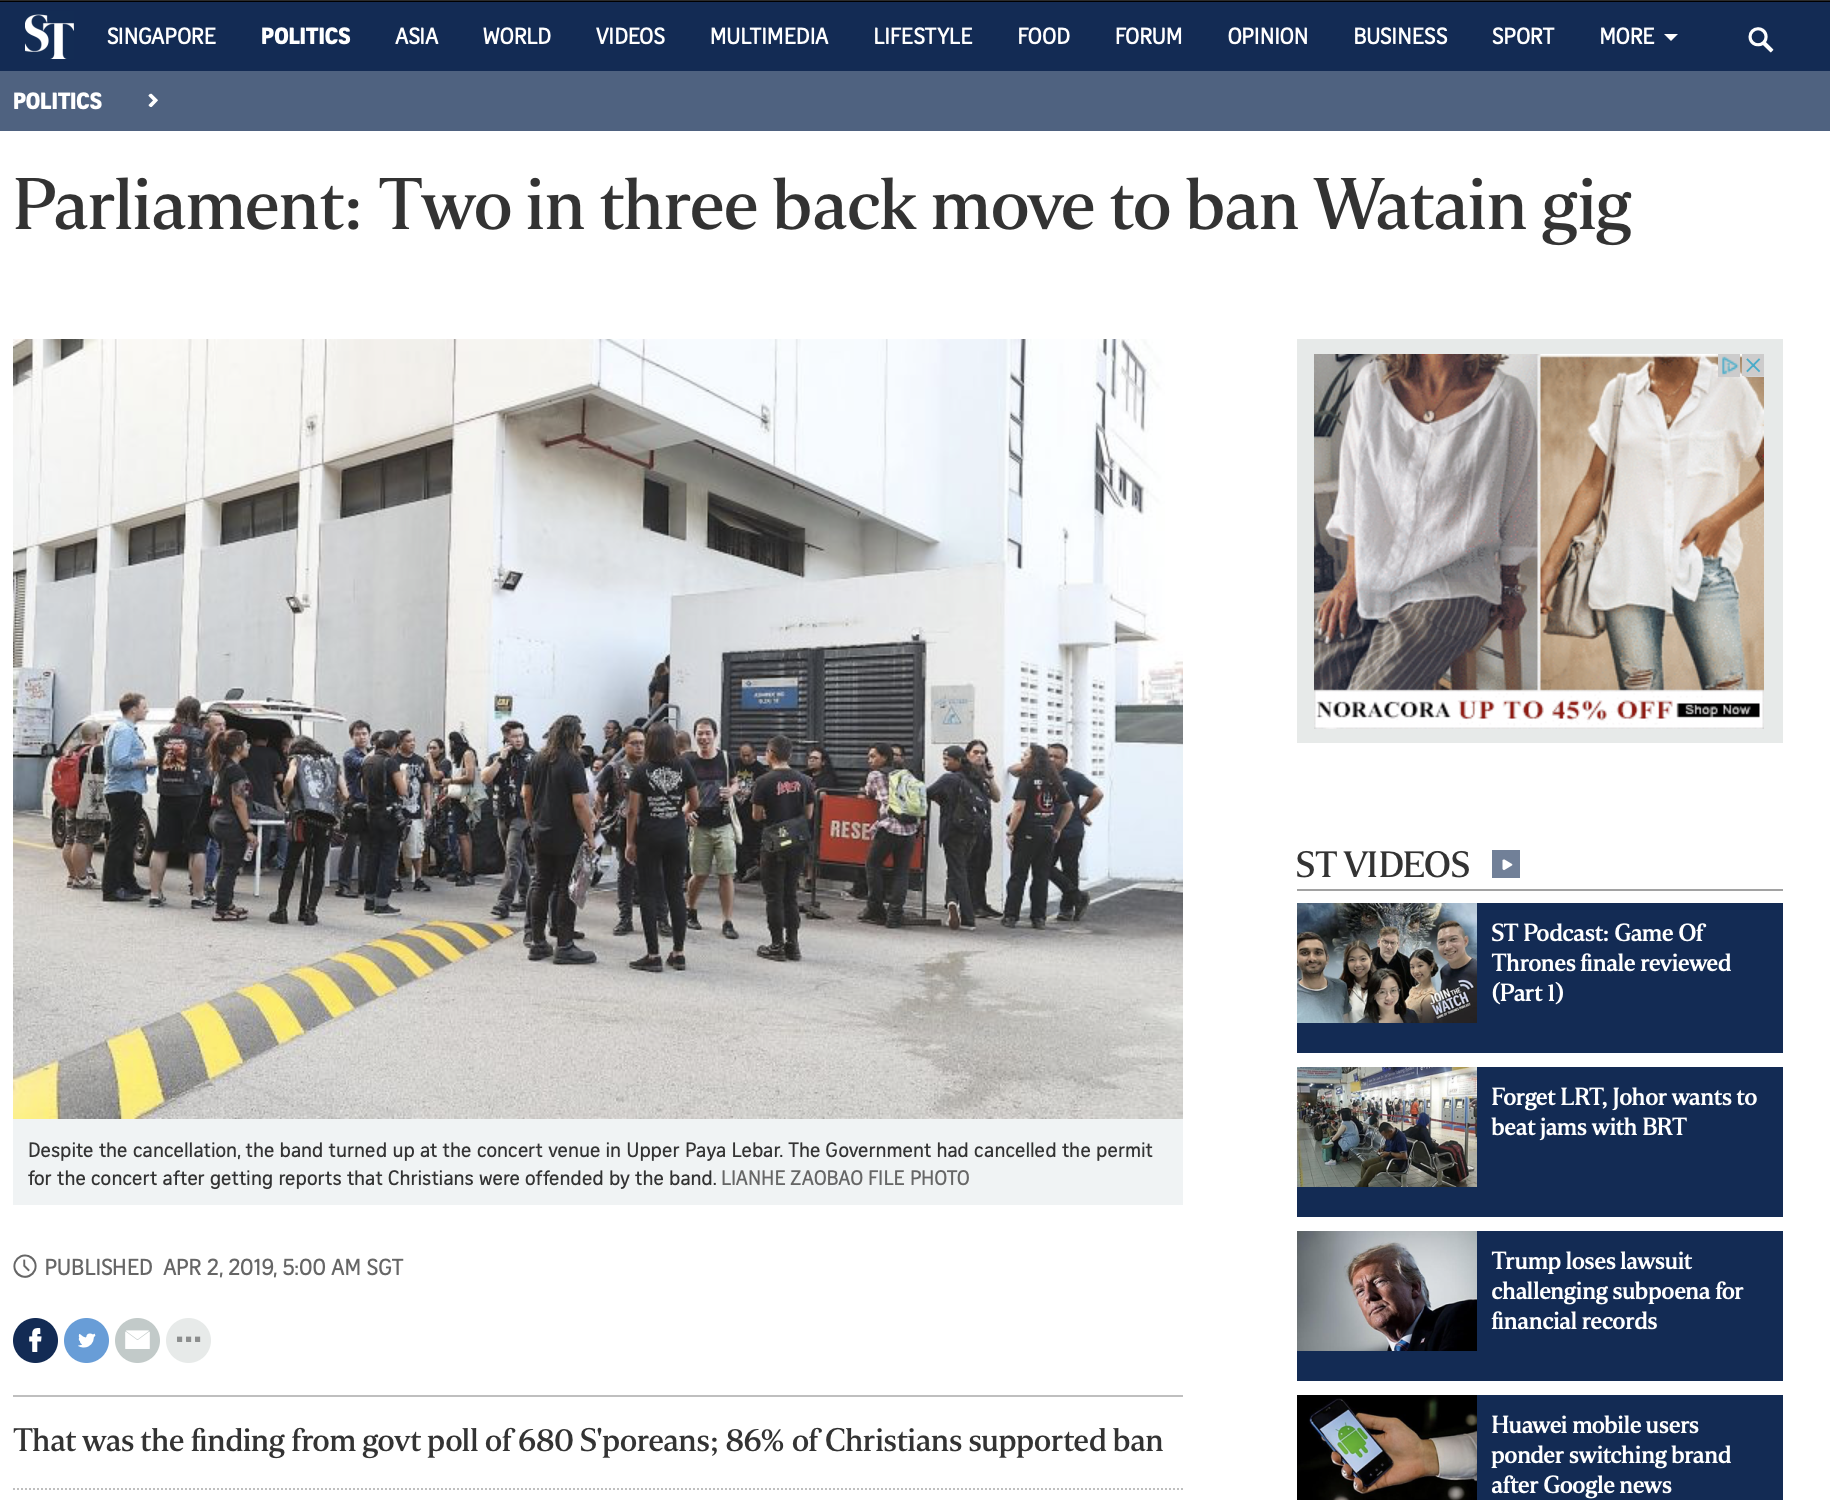
\includegraphics[width=0.8\linewidth]{images/STwatain} 

}

\caption{Screenshot of online article on results from REACH poll. Retrieved May 21, 2019.}\label{fig:st-watain}
\end{figure}

The next day, national newspaper The Straits Times ran
\href{https://www.straitstimes.com/politics/singapolitics/parliament-two-out-of-three-singaporeans-back-governments-move-to-cancel}{a
story} headlined ``Parliament: Two in three back move to ban Watain
gig''. Within the text of the article, it reads:

\begin{quote}
The Government decided to cancel the permit for Watain's concert last
month when it received reports that mainstream Christians were very
concerned and offended by the band, Home Affairs Minister K. Shanmugam
said yesterday. \textbf{And a survey of Singaporeans by government
feedback unit Reach found that two in three supported the move, he
noted.} Among Christians, 86 per cent were supportive of the move to
disallow the concert, the Reach poll found.
\end{quote}

Note the qualifier ``among those who were aware'' is neither in the
headline (Figure \ref{fig:st-watain}) nor the body of the
article\footnote{CNA ran a similar headline, but included the qualifier
  within the article. See
  \url{https://www.channelnewsasia.com/news/singapore/2-in-3-singaporeans-in-reach-poll-supported-government-s-11401066}}.
\emph{Why is this important?}
\href{https://www.reach.gov.sg/~/media/2019/press-release/findings-of-poll-on-watain-concert--1-april-2019.pdf}{Results
from REACH} show that 63\% of respondents were aware, and \emph{out of
these respondents}, 64\% supported the government's ban. This means that
out of \emph{all} respondents to the survey, only about 40\% reported
supporting the ban. This means that the qualifying phrase ``among those
who were aware'' meaningfully changes the interpretation of the results
- we shouldn't be able to say that \textbf{the majority of Singaporeans}
supported the ban when in fact only 40\% of the survey respondents did
so.

In effect, the Straits Times article is invoking a strong assumption
here (see \ref{ooptech} for a more technical explanation) - that
\emph{if} those who were unaware were in fact able to express their
support for the ban, the same proportion of respondents (among those who
were aware, 64\%) would also support the ban. But being aware of the ban
is a \emph{prerequisite} for support of the ban, which makes this
assumption rather unreasonable. Even assuming this hypothetical scenario
were possible, the actual figure could be higher or lower - it depends
on how similar (or different) the unaware are to the aware. Those who
were not aware may be less likely to care about black metal music (or
simply too busy to keep up with current affairs) and simply base their
support of the ban on their general sentiment toward government
policies. This seemingly minor omission of the qualifier can lead to
false conclusions pretty quickly. Let us look at another example.

\section{Media claim 2: Web-savvy Seniors}\label{websavvy}

Part of my research involves looking at how Internet use can improve the
lives of older adults \citep[see][]{ang_going_2018}. I was interested in
what the overall situation was like in Singapore, and googled something
like ``internet use seniors''. One 2014 article in the Straits Times
immediately caught my eye (see Figure \ref{fig:st-websavvyseniors}).

\begin{figure}

{\centering 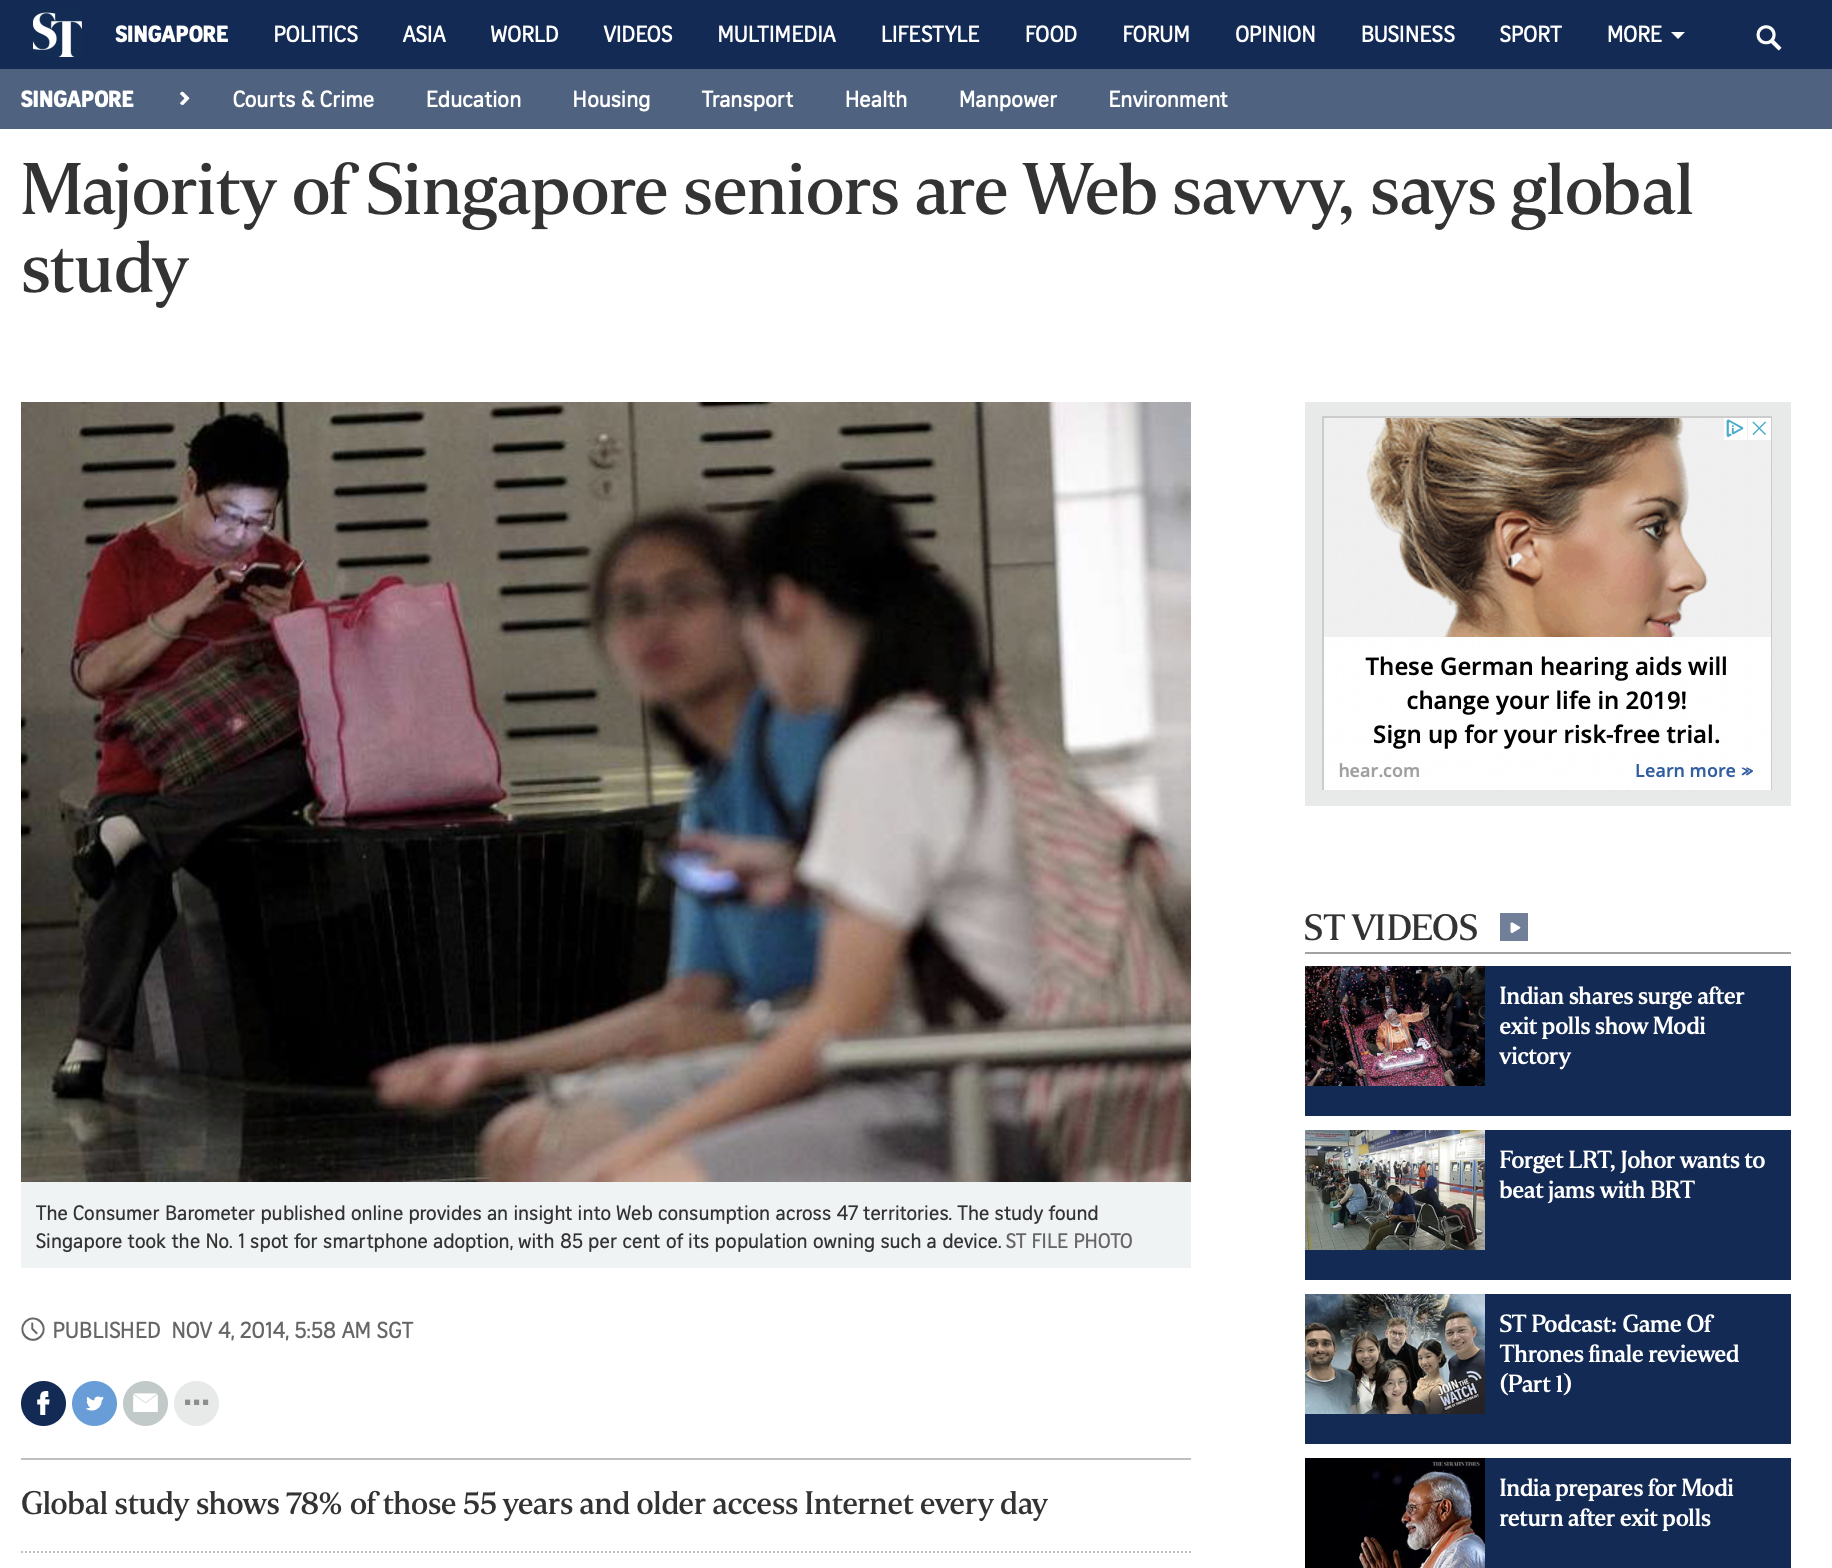
\includegraphics[width=0.8\linewidth]{images/STwebsavvyseniors} 

}

\caption{Screenshot of online article on web-savvy seniors. Retrieved May 21, 2019.}\label{fig:st-websavvyseniors}
\end{figure}

Within the article, the reporter states:

\begin{quote}
Also, 78 per cent of those aged 55 and older here access the Internet
every day either via the traditional Web browser or smartphone apps,
putting Singapore fifth in the world for having the most Internet-savvy
seniors.
\end{quote}

I was skeptical. Over and above my anecdotal experience with Singapore
older adults, past research in the United States\footnote{For instance,
  see
  \url{https://www.pewinternet.org/2012/06/06/older-adults-and-internet-use/}}
gave me reason to expect that the proportion of older people even using
the Internet (everyday or not) should be much lower. Some results from
Consumer Barometer are available online, so we can
\href{https://www.consumerbarometer.com/en/trending/?countryCode=SG\&category=TRN-AGE-55-PLUS}{check
for ourselves}. Of interest in Figure \ref{fig:cb-seniorsinternet} are
numbers reflecting internet use in year 2014, which is when the news
article was published. Note that the percent of Singaporeans aged 55 and
above who use the internet daily in 2014 \textbf{is 29\%, not 78\% as
the article suggests.}

\begin{figure}

{\centering 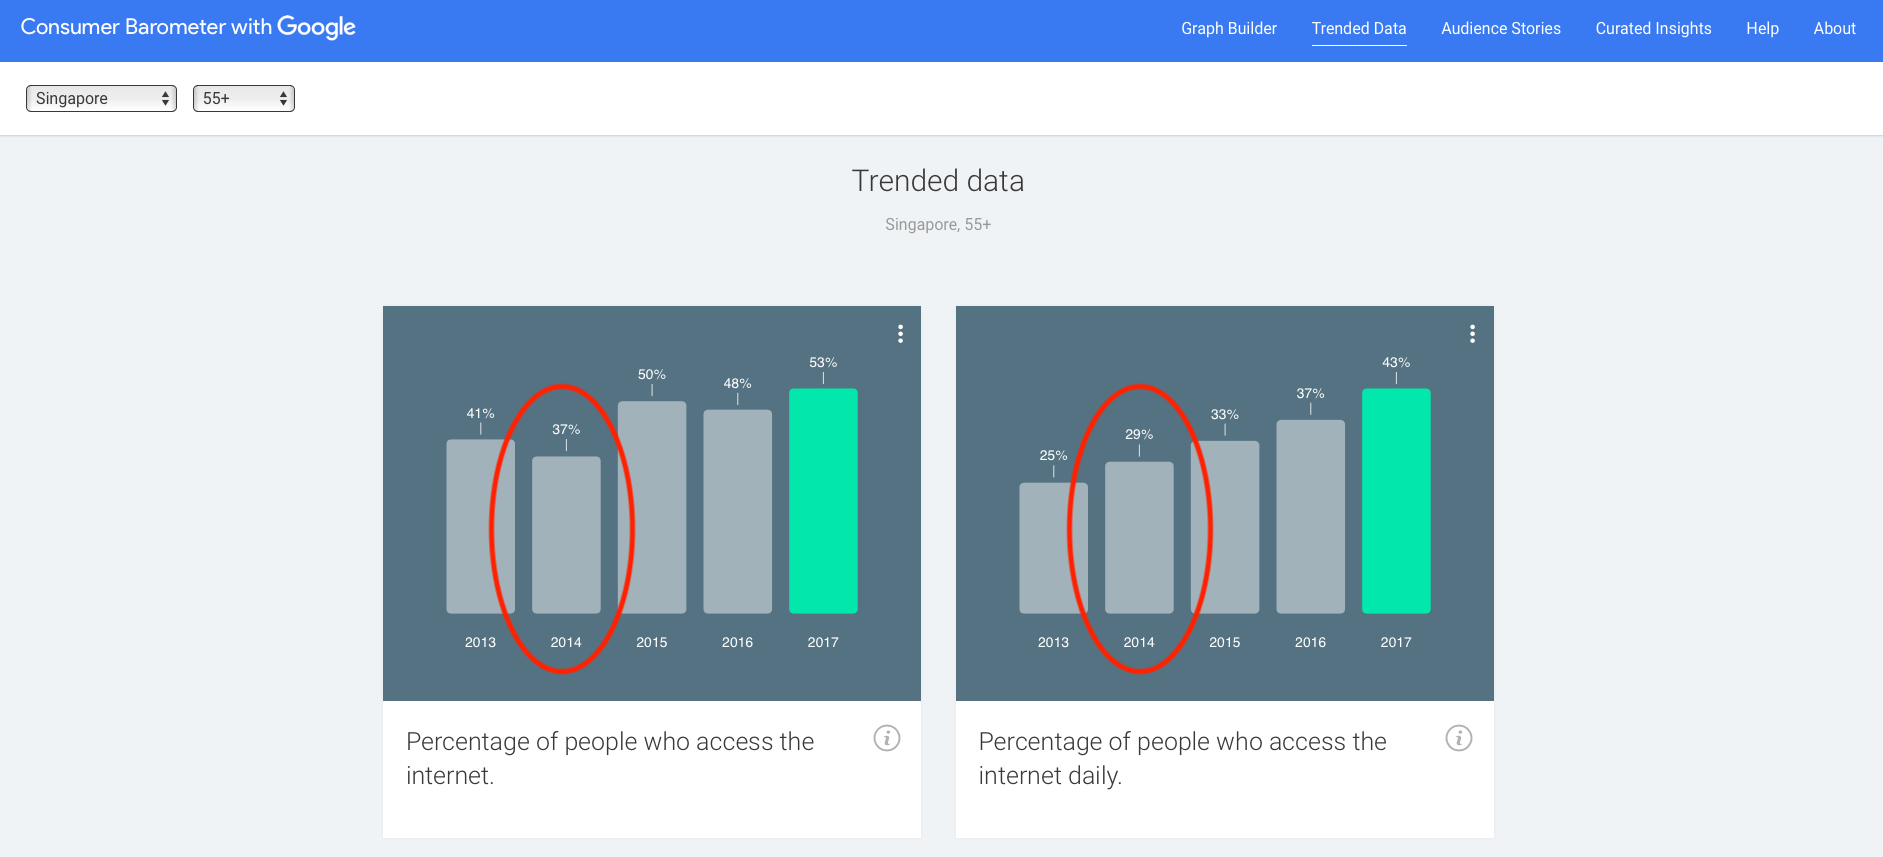
\includegraphics[width=1\linewidth]{images/CBseniorsinternet} 

}

\caption{Screenshot of Consumer Barometer findings across time. Retrieved May 21, 2019.}\label{fig:cb-seniorsinternet}
\end{figure}

How then, did the reporter get things so wrong? While detailed
statistics for 2014 doesn't seem available online anymore, a little
investigation using 2017 figures shows how the reporter arrived at a
number as high as 78\%.

\begin{figure}

{\centering 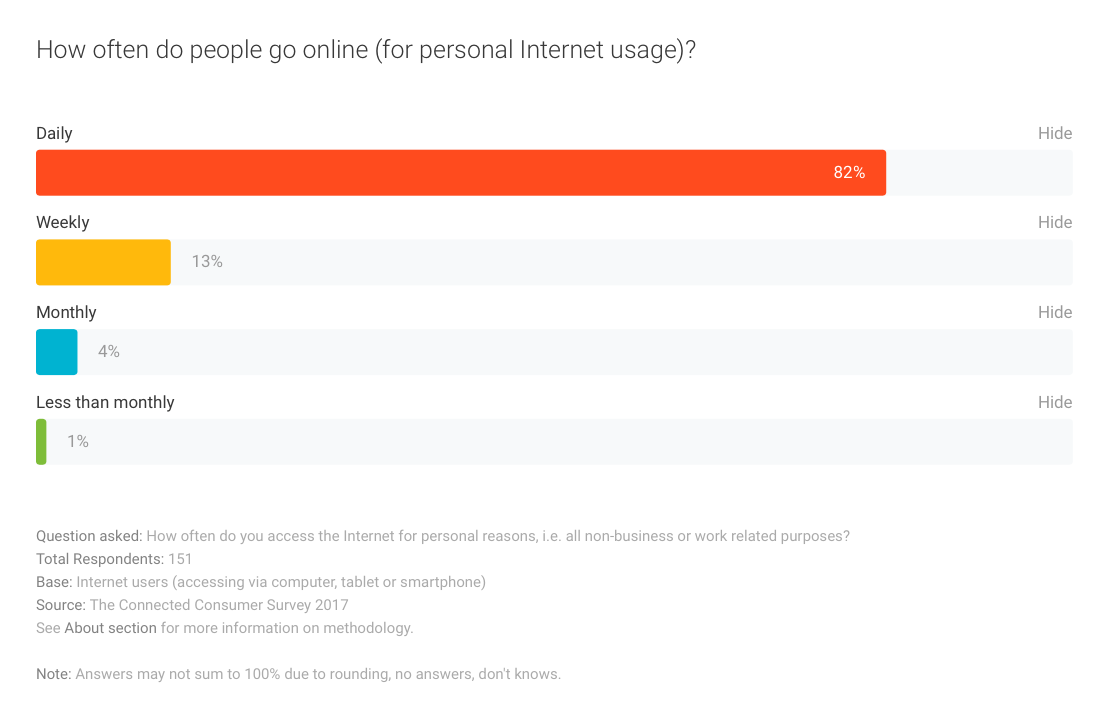
\includegraphics[width=0.9\linewidth]{images/CBsinglequestion} 

}

\caption{Screenshot of Consumer Barometer results on 2017 internet use. Retrieved May 21, 2019.}\label{fig:cb-single}
\end{figure}

Looking at Figure \ref{fig:cb-single}, the crucial part is the footnote
that says ``base'', which tells us that the 82\% figure for daily
Internet usage in 2017 are \textbf{among those who use the internet}. We
can easily calculate this 82\% ourselves by using the numbers in Figure
\ref{fig:cb-seniorsinternet} - note that 43\% is approximately 82\% of
53\%. That is, \(\frac{43}{53} \approx 0.82\). Using the same strategy,
we can recover the reporter's figure for 2014:
\(\frac{29}{37} \approx 0.78\).

\emph{What does this mean?} This means that just like the reporter in
the Watain example (\ref{watain}), this reporter left out an important
qualifier - only 29\% of all older adults in Singapore use the internet
daily, but 78\% \textbf{of those who use the internet} use it daily.
This vast discrepancy is highly consequential - the statement that ``78
per cent of those aged 55 and older here access the Internet every day''
is false, and the headline that ``Majority of Singapore seniors are Web
savvy'' is misleading at best.

\section{Technical Appendix}\label{ooptech}

Before we go into a more technical explanation of what went wrong in
these two cases, let us first move from proportions to probabilities.
The difference between a proportion and a probability is important here.
Note that when Minister Shanmugam asserted the REACH poll provided
evidence that the Government's ``assessment of public sentiment turned
out to be correct'', he was not suggesting that 680 Singaporeans form
the whole Singapore public. The underlying assumption was that since
most survey respondents (who were aware) supported the ban, it is likely
that most Singaporeans (who are aware) will also support the ban. That
is, he was using the \emph{proportion} of supportive survey respondents
(a description of the sample), to infer the \emph{probability} (a
hypothetical quantity) of any one Singaporean supporting the ban.

The difference between a probability and a proportion may be simplified
using a coin flip example. If I flip a fair coin 4 times, the proportion
of heads may be 0, 0.25, 0.5, 0.75, or 1. However, since it is a fair
coin, the probability of getting a heads is, by definition, 0.5. So the
proportion may or may not equal the probability. What we know is that
the more times I flip the coin, the more likely the proportion of heads
will reflect the true probability of getting a heads. It is thus common
to hear people say that the probability is the ``long-run proportion of
an event''. Below is some code (in R) for you to try out the coin flip
example.

\begin{Shaded}
\begin{Highlighting}[]
\CommentTok{# Set the number of trials to 4. }
\CommentTok{# You may change the number to see what happens.}
\NormalTok{n <-}\StringTok{ }\DecValTok{4} 
\CommentTok{# Get the proportion of heads after flipping a fair coin n times. }
\CommentTok{# Try this a few times.}
\KeywordTok{sum}\NormalTok{(}\KeywordTok{rbinom}\NormalTok{(n, }\DecValTok{1}\NormalTok{, }\DataTypeTok{prob=}\FloatTok{0.5}\NormalTok{))}\OperatorTok{/}\NormalTok{n }
\end{Highlighting}
\end{Shaded}

We have now established that the main reason why we are interested in
proportions from a REACH poll is because they purport to tell us
something about Singaporeans in general. That is, the REACH poll
suggests that if we were to randomly pick a Singaporean from those who
are aware of the ban), the probability of this person supporting the ban
is about 0.64 (or 64\%). The problem at hand then reduces to a trivial
probability question, assuming that we all remember basic probability
rules from secondary (primary?) school\footnote{Or that we can Google it
  if not}. If the REACH poll is indeed representative of all
Singaporeans, then we have the following quantities:

 \[
\begin{aligned}
&\Pr(\text{Aware of Ban}) = 0.63 \\
&\Pr(\text{Not Aware of Ban}) = 1 - \Pr(\text{Aware of Ban}) = 0.37 \\
&\Pr(\text{Support Ban } | \text{ Aware of Ban}) = 0.64 
\end{aligned}
\]

\(\Pr(\text{Support Ban } | \text{ Aware of Ban})\) is a conditional
probability, but the quantity that is being asserted in the news article
is \(\Pr(\text{Support Ban})\), which is the total probability. Using
the law of total probability, we know that:

 \[
\begin{aligned}
\Pr(\text{Support Ban}) &= \Pr(\text{Support Ban } | \text{ Aware of Ban})\cdot \Pr(\text{Aware of Ban}) \\
& \quad + \Pr(\text{Support Ban } | \text{ Not Aware of Ban})\cdot \Pr(\text{Not Aware of Ban}) 
\end{aligned}
\]

Plugging in the numbers that we have,

 \[
\begin{aligned}
\Pr(\text{Support Ban}) &= 0.64 \cdot 0.63 + \Pr(\text{Support Ban } | \text{ Not Aware of Ban}) \cdot 0.37 \\
\end{aligned}
\]

we see that \(\Pr(\text{Support Ban}) = 0.64\) if and only if
\(\Pr(\text{Support Ban } | \text{ Not Aware of Ban})\) also equals
\(0.64\). That said,
\(\Pr(\text{Support Ban } | \text{ Not Aware of Ban})\) is logically
impossible, and should equal zero. Similarly, for the Web-savvy Seniors
example,

 \[
\begin{aligned}
\Pr(\text{Use Internet Daily}) &= \Pr(\text{Use Internet Daily } | \text{ Use Internet})\cdot \Pr(\text{Use Internet}) \\
& \quad + \Pr(\text{Use Internet Daily } | \text{ Don't Use Internet})\cdot \Pr(\text{Don't Use Internet}) \\
&= 0.78 \cdot 0.37 + \Pr(\text{Use Internet Daily } | \text{ Don't Use Internet})\cdot 0.63 \\
\end{aligned}
\]

where \(\Pr(\text{Use Internet Daily } | \text{ Don't Use Internet})\)
is impossible and should be zero. In both cases, total probabilites are
substantially different from the conditional probabilities, and there is
no reason to believe they would be the same.

\section{Conclusion}\label{conclusion}

By now, it should be clear that qualifiers attached to proportions (and
percentages) are critical. Without them, results from studies can be
blown out of proportion. It is not wise to completely rely on assertions
made by news articles (or other kinds of reports), even from supposedly
credible agencies like the Straits Times. As we have seen, social
scientists should be comfortable with interpreting data from its
source\footnote{This, however, first requires data to be made available
  for replication purposes.} in order to evaluate claims that are being
made in public discourse today.

\chapter{Case study 2}\label{case2}

\begin{verbatim}
Contributor:
Date:
\end{verbatim}

Another case study goes here. Do you wish to contribute?

This is an example of in-line code annotation and output.

\begin{Shaded}
\begin{Highlighting}[]
\KeywordTok{par}\NormalTok{(}\DataTypeTok{mar =} \KeywordTok{c}\NormalTok{(}\DecValTok{4}\NormalTok{, }\DecValTok{4}\NormalTok{, .}\DecValTok{1}\NormalTok{, .}\DecValTok{1}\NormalTok{))}
\KeywordTok{plot}\NormalTok{(pressure, }\DataTypeTok{type =} \StringTok{'b'}\NormalTok{, }\DataTypeTok{pch =} \DecValTok{19}\NormalTok{)}
\end{Highlighting}
\end{Shaded}

\begin{figure}

{\centering 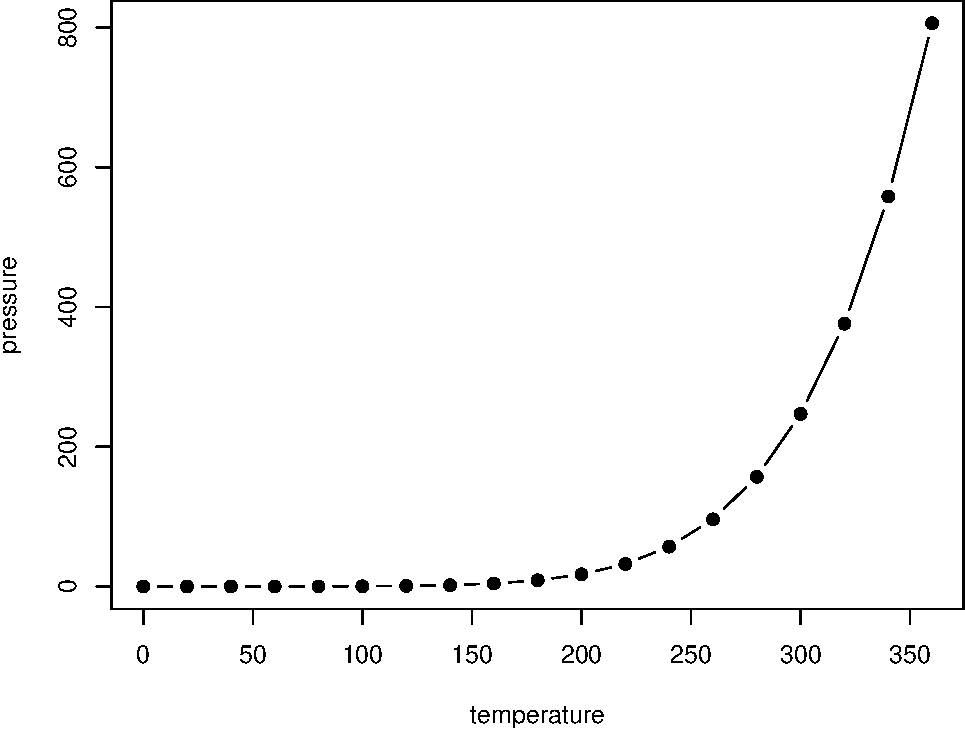
\includegraphics[width=0.8\linewidth]{bookdown_files/figure-latex/nice-fig-1} 

}

\caption{Here is a nice figure!}\label{fig:nice-fig}
\end{figure}

Figures can be referenced, e.g., see Figure \ref{fig:nice-fig}.
Similarly, you can reference tables generated from
\texttt{knitr::kable()}, e.g., see Table \ref{tab:nice-tab}.

\begin{Shaded}
\begin{Highlighting}[]
\NormalTok{knitr}\OperatorTok{::}\KeywordTok{kable}\NormalTok{(}
  \KeywordTok{head}\NormalTok{(iris, }\DecValTok{5}\NormalTok{), }\DataTypeTok{caption =} \StringTok{'Here is a nice table!'}\NormalTok{,}
  \DataTypeTok{booktabs =} \OtherTok{TRUE}
\NormalTok{)}
\end{Highlighting}
\end{Shaded}

\begin{table}[t]

\caption{\label{tab:nice-tab}Here is a nice table!}
\centering
\begin{tabular}{rrrrl}
\toprule
Sepal.Length & Sepal.Width & Petal.Length & Petal.Width & Species\\
\midrule
5.1 & 3.5 & 1.4 & 0.2 & setosa\\
4.9 & 3.0 & 1.4 & 0.2 & setosa\\
4.7 & 3.2 & 1.3 & 0.2 & setosa\\
4.6 & 3.1 & 1.5 & 0.2 & setosa\\
5.0 & 3.6 & 1.4 & 0.2 & setosa\\
\bottomrule
\end{tabular}
\end{table}

\bibliography{book.bib,packages.bib,zotero.bib}


\end{document}
